\documentclass{sig-alternate-05-2015}
	\pdfpagewidth=8.5truein
	\pdfpageheight=11truein

\usepackage{graphicx}
\usepackage{subfig}
\usepackage[bookmarks=false]{hyperref}
\usepackage{xspace}
\usepackage{listings}
\usepackage[usenames, dvipsnames]{color}

\usepackage{booktabs}         

\graphicspath{{./img/}}

%\hyphenation{op-tical net-works semi-conduc-tor}

%
\def\sharedaffiliation{%
\end{tabular}
\begin{tabular}{c}}
%

\lstset{language=Python}

\definecolor{LightGray}{RGB}{250,250,250}

\lstdefinestyle{custompython}{
	captionpos=b,                    % sets the caption-position to bottom
	% frame=tb,
	xleftmargin=\parindent,
	language=Python,
	basicstyle=\footnotesize\ttfamily,
	keywordstyle=\bfseries\color{MidnightBlue},
	morekeywords={*,python,times,test_folder,url},
	stringstyle=\color{PineGreen},
  	commentstyle=\color{Magenta},
  	backgroundcolor=\color{LightGray}
}


\newcommand{\tool}{Flask Dashboard\xspace}
\newcommand{\zee}{Zeeguu\xspace}
\newcommand{\git}{\texttt{git}\xspace}
\newcommand{\install}{{\small \texttt{pip install flask\_monitoring\_dashboard}}\xspace}
\newcommand{\activeUserCount}{two hundred\xspace}
\newcommand{\code}[1]{\texttt{#1}\xspace}
\newcommand{\perspective}[1]{{\bf {\small {\texttt{#1}}\xspace}}}

\newcommand{\lesson}[1]{{\bf {\small {\texttt{Lesson: }}\xspace}}: #1}

\usepackage{fourier-orns}

\definecolor{myred}{RGB}{230, 20, 70}
\definecolor{mygreen}{RGB}{60, 180, 75}
\definecolor{uploadUserData}{RGB}{135, 143, 197}
\definecolor{feedItems}{RGB}{245, 130, 48}


\newcommand{\niceseparator}
	{
		\begin{center}
  		% $\ast$~$\ast$~$\ast$
  		% $\clubsuit$~$\clubsuit$~$\clubsuit$
  		\leafleft
		\end{center}
	}

% Endpoint Names 
%\newcommand{\epDecoration}[1]{{\small {\bf #1}}\xspace}
\newcommand{\epDecoration}[1]{\code{#1}}

\newcommand{\epColorDecoration}[2]{\color{#1}$\blacksquare$\color{black}\code{#2}}

\newcommand{\epTranslations}{{\epColorDecoration{myred}{api.get\_possible\_translations}}\xspace}
\newcommand{\epOutcome}{\epColorDecoration{mygreen}{api.report\_exercise\_outcome}}
\newcommand{\epFeedItems}{\epColorDecoration{feedItems}{api.get\_feed\_items\_with\_metrics}}
\newcommand{\epUserActivity}{\epColorDecoration{uploadUserData}{api.upload\_user\_activity\_data}}


% Author Comments / Discussion

\definecolor{mlcolor}{RGB}{140, 140, 205}
\definecolor{vacolor}{RGB}{255, 0, 255}

\newcommand{\ml}[1]{ 
	{\footnotesize \color{mlcolor}ML: #1}
	}

\newcommand{\ins}[1]{ 
	{\color{blue}#1}
	}


\newcommand{\va}[1]{ 
	{\footnotesize \color{vacolor}VA: #1}
}


\newcommand{\mltp}[1]{\ml{Thijs, Patrick: #1}}
\newcommand{\mlv}[1]{\ml{Vasilios: #1}}

\definecolor{todocolor}{RGB}{200, 140, 200}

\newcommand{\todo}[1]{ 
	{\bfseries \color{todocolor}Todo: #1}
	}

\newcommand{\Fref}[1]{Fig.~\ref{#1}}
\newcommand{\Sref}[1]{Sec.~\ref{#1}}




\begin{document}
	
\CopyrightYear{2018}
\setcopyright{acmcopyright}
\conferenceinfo{SAC 2018,}{April 09-13, 2018, Pau, France}
%\isbn{978-1-4503-5191-1/18/04}\acmPrice{\$15.00}
%\doi{DOI: http://dx.doi.org/xxx}
	
	
%
\title{A Low-Effort Analytics Platform for Visualizing Evolving Flask-Based Python Web Services}
% Alternative Titles: The Importance of Visualization in the Performance Monitoring of Python Web Services


\numberofauthors{4}
\author{
\alignauthor Patrick Vogel\\
\email{p.p.vogel@student.rug.nl}
%
\alignauthor Thijs Klooster\\
\email{t.klooster.1@student.rug.nl}
%
\and
\alignauthor Vasilios Andrikopoulos\\
\email{v.andrikopoulos@rug.nl}
%
\alignauthor Mircea Lungu\\
\email{m.f.lungu@rug.nl}
%
\sharedaffiliation
\affaddr{Johann Bernoulli Institute for Mathematics and Computer Science}\\
\affaddr{University of Groningen, the Netherlands}\\
}
\date{\today}

% make the title area
\maketitle

\begin{abstract}
\todo{Update abstract \& title}
  Tens of thousands of web applications are written in Flask, a Python-based web framework. Despite a rich ecosystem of extensions, there is none that supports the developer in gaining insight into the evolving performance of their service. In this paper, we introduce \tool, a library that addresses this problem. We present the ease with which the library can be integrated in an already existing web application, discuss some of the visualization perspectives that the library provides and point to some future challenges for similar libraries.

\end{abstract}

\begin{CCSXML}
	<ccs2012>
	<concept>
	<concept_id>10010520.10010553.10010554</concept_id>
	<concept_desc>Computer systems organization~Robotics</concept_desc>
	<concept_significance>100</concept_significance>
	</concept>
	<concept>
	<concept_id>10003033.10003083.10003095</concept_id>
	<concept_desc>Networks~Network reliability</concept_desc>
	<concept_significance>100</concept_significance>
	</concept>
	</ccs2012>  
\end{CCSXML}

\ccsdesc{Computer systems organization~Robotics}
\ccsdesc[100]{Networks~Network reliability}



\section{Introduction}

\todo{Intro to be rewritten; refer to VISSOFT paper as previous work, explain focus is on integration with version control/CI for evolution support, and use of unit tests as early performance indicator}

\todo{motivate with: monitoring in a world which is becoming more and more service-oriented is essential because it allows to perform three main types of actions: system adaptations to provide the request service at the desired level of quality, enabling flexibility in dealing with changing requirements and modes of operation, and enabling operational awareness through dashboards organizing the collected data~\cite{pernici2016monitoring}. In this work we focus on the last part and we discuss how a minimal effort probe-based solution for a particular type of web services can be used to facilitate the other two types of actions by involving the developer.}

\todo{explain: in~\cite{vogel2017low} we introduced the \tool an a high level with a focus on presenting its performance visualization aspects; in this work we only summarize these features by means of introducing some of the provided functionalities of the \tool. We focus on discussing how the tool is implemented and operating, provide a deeper look at its capabilities for integration with version control and continuous integration environments, introduce a mechanism for performance prediction, and provide an evaluation of the proposed approach based on a case study. }

%Every system is a distributed system nowadays \cite{cavage2013there}. Indeed a very large number of applications and web applications are nowadays implemented as two-tier architectures with a front-end implemented with web technologies and a service back-end.
%\ml{I'm not completely happy with this paragraph}
{\em There is no getting around it: you are building a distributed system} argues a recent article \cite{cavage2013there}. Indeed, even the simplest second-year student project is a web application implemented as two-tier architecture with a Javascript/HTML5 front-end a service backend, usually a REST API.

% \hfill mds
% Many contemporary programming languages are offering libraries, modules, or frameworks that facilitate the development of such architectures. 
Python is one of the most popular programming language choices for implementing the back-end of web applications. GitHub contains more than 500K open source Python projects and the Tiobe Index\footnote{TIOBE programming community index is a measure of popularity of programming languages, created and maintained by the TIOBE Company based in Eindhoven, the Netherlands} ranks Python as the 4th most popular programming language as of June 2016.
 
% possible flask summary
Within the Python community, Flask\footnote{\url{http://flask.pocoo.org/}} is a very popular web framework\footnote{More than 25K projects on GitHub (5\% of all Python projects) are implemented with Flask (cf. a GitHub search for ``language:Python Flask'')}. It provides simplicity and flexibility by implementing a bare-minimum web server, and thus advertises as a micro-framework. The Flask tutorial shows how setting up a simple Flask {\em ``Hello World''} web-service requires no more than 5 lines of Python code \cite{ flask:tutorial}.
% end of summary
 
Despite their popularity, to the best of our knowledge, there is no simple solution for monitoring the evolving performance of Flask web applications. Thus, every one of the developers of these projects faces one of the following options when confronted with the need of gathering insight into the runtime behavior of their implemented services: 

  \begin{enumerate}

    \item Use a commercial monitoring tool which treats the subject API as a black-box (e.g. Pingdom, Runscope). 
    % , Graphite+Graphana+statd etc.

    \item Implement their own ad-hoc analytics solution, having to reinvent basic visualization and interaction strategies. 

    \item Live without analytics insight into their services.

  \end{enumerate}

%\todo{For the first point in the list, we can also argue that analytics solutions like Google Analytics can be used, but they have no notion of versioning/integration with the development life cycle. Feel free to cite \cite{papazoglou2011managing} for service evolution purposes}

For projects on a budget (e.g. research, startups) the first and the second options are often not available due to time and financial constraints. Even when using 3rd-party analytics solutions, a critical insight into the evolution of the exposed services of the web application, is missing because such solutions have no notion of versioning and no integration with the development life cycle.~\cite{papazoglou2011managing}

To avoid projects ending up in the third situation, that of living without analytics, in this paper we present \tool~ --- a low-effort service monitoring library for Flask-based Python web services that is easy to integrate and enables the {\em agile assessment} of service evolution. \cite{Nier12b}

As a case study, on which we will illustrate our solution, we are going to use an open source API which, for several years, was in the third of the above-presented situations.

% In the next section, we will present a case study of an open source research API which was for a long time in the third situation presented above -- deployed without analytics insight.

\todo{Add signposting paragraph}

\section{Case Study}
\label{sec:case}

%\todo{Either leave as is or add more info on usage by college if possible}

  \zee\footnote{\url{https://github.com/zeeguu-ecosystem/}} is a platform and an ecosystem of applications for accelerating vocabulary acquisition in a foreign language \cite{Lungu16}. 
%
  The architecture of the ecosystem has at its core an API and a series of satellite applications that together offer to a learner three main inter-dependent features:

  \begin{enumerate}

    \item Reader applications that provide effortless translations for those texts which are too difficult for the readers.

    \item Interactive exercises personally generated based on the preferences and past likes of the learner.

    \item Article recommendations which are personalized for the interests of the learner and come with difficulty estimation that helps the learner find articles with the appropriate difficulty.

  \end{enumerate}

  The core API implemented with Flask and Python provides correspondingly three types of functionality: contextual translations, article recommendations, and personalized exercise suggestions. In total the API provides a bit less than 50 endpoints, out of which probably a dozen are very frequently used. 
  % The development of the core API itself is a research project. 

  At the time of writing this article, the ecosystem consists of a reader web application, a web based exercises platform, and a smartwatch application, which are used at the moment of writing this article by more than \activeUserCount active users. The users come from a highschool, a language school, and some users are using it on their own, without any educational context. The highest load we observed until now on the API consisted of 12K requests in one day.

  
  We will use this \zee API as a case study for this paper. 
  All the figures in this paper are captured from the actual deployment of \tool in the context of the \zee API. The figures are interactive offering basic data exploration capabilities: filter, zoom, and details on demand\cite{Shne99a}. The \tool deployment for the case study can be accessed publicly\footnote{\url{https://zeeguu.unibe.ch/api/dashboard}; username: {\em guest}, password: {\em soap-sac}}. 

 % \todo{create new account, update URL if necessary, update activeUserCount, add a couple of sentences of the current state of the case study with the college/language center}
% \ml{we should consider adding also one section in which the architecture/implementation and main features of the dashboard are presented before going on with discussing them in more depth in the following sections --- this should include a rundown on which views are provided from where (overview or per endpoint)}



\section{The Flask Dashboard}
\label{sec:tool}

%\todo{Refer to VISSOFT paper~\cite{vogel2017low} and rephrase where possible; add more info on implementation, e.g. annotation mechanism, database design, session handling etc.}

  As discussed in the introductory section, in previous work~\cite{vogel2017low} we introduced \tool, a drop-in Python library that allows developers to monitor their Flask-based Python web applications with minimal effort.
%
  The \tool is implemented for Python 3.6 and is available on the Python Package Index repository\footnote{\url{https://pypi.python.org/pypi/flask-monitoring-dashboard/1.8}} from where it can be installed by running \install from the command line. 
%  
  The source code of the \tool is published under a permissive MIT license and is available on GitHub\footnote{\url{https://github.com/flask-dashboard}}.
  
  \paragraph{Usage \& Configuration}
  
  The fact that the \tool itself is being developed in Python using Flask makes binding to the services of a to-be monitored application developed with the same technologies easy and intuitive. \ml{this is not what matters... rather, what matters is that with the right backend, we can do this minimal configuration for any technology... do you see what i mean? let me see if i can put it in words...}

  Our main goal with the \tool was to allow the integration of the dashboard with an API with minimal effort.
  To start using the \tool, one simply needs to add two lines of code to their Flask web service\footnote{\ins{ In this paper we present the integration with APIs written in Python and Flask hoping that this will not prevent the reader from seeing the more general idea; all the tools we show here for Flask can be applied to other API technologies (e.g. Django) by simply providing a few back-end adapters in the right places. }}:

  % caption=Configuring the \tool is straightforward,
  \begin{lstlisting}[style=custompython]
  import dashboard

  # flask_app is the Flask app object
  dashboard.bind(flask_app)
  \end{lstlisting}

  After (re)deployment of the application, the \tool becomes available at the \code{/dashboard} route of the Flask application. Further configuration is possible by adding additional statements before the binding definition, for example,

  \begin{lstlisting}[style=custompython]
  ...
  dashboard.config.link = 'mydashboard'
  dashboard.bind(flask_app)
  \end{lstlisting}
  
  allows for a custom route (\code{/mydashboard}) to the dashboard to be defined by the programmer. An external configuration file can be used instead, or in addition to this:
  
  \begin{lstlisting}[style=custompython]
  ...
  dashboard.config.from_file('config.cfg')
  ...
  \end{lstlisting}

  During binding, the \tool will search for all endpoints defined in the target application. These will be presented to the user in the tool web interface, where the user can select the ones that should be monitored, see \Fref{fig:sep}. The last access time of the endpoint by users, irrespective of whether it is selected by the user to be monitored or not, is also displayed as the means of identifying potentially obsolete endpoints.

    % \mltp{a small screenshot of how the dashboard allows one to select the interesting }
    \begin{figure}
      \centering
      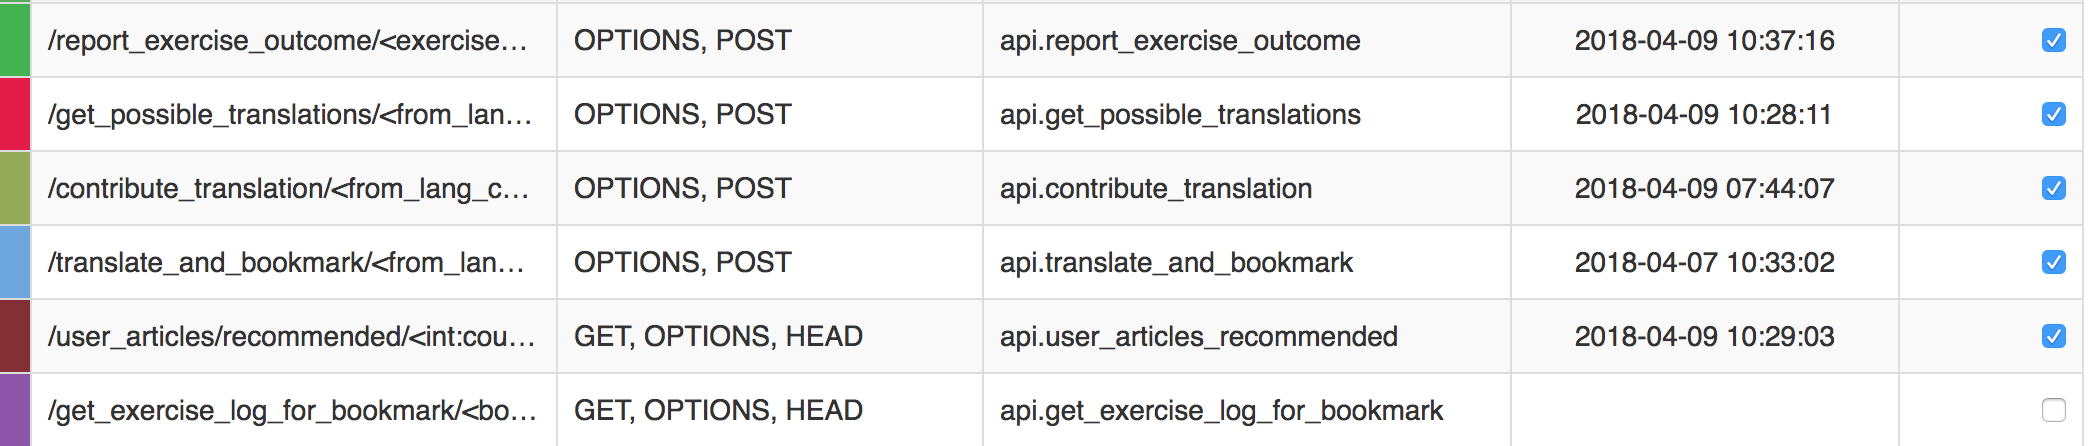
\includegraphics[width=\linewidth]{selecting_endpoints.png}
      \caption{Endpoints that are available for monitoring in the \zee API}
      \label{fig:sep}
    \end{figure}

  In order to monitor an endpoint, the \tool creates a function wrapper for the API function that corresponds to the endpoint. This way, the wrapper will be executed whenever that API call is made. The wrapper contains the code that takes care of monitoring an endpoint. Data collected by the wrappers are persisted in a local database. The SQLAlchemy Object Relational Mapper\footnote{\url{https://www.sqlalchemy.org/}} on top of SQLite\footnote{\url{https://www.sqlite.org/}} is used for this purpose.

  \ml{we must insert at least one dashboard view here... otherwise people will lose their patience... also it will help with explaining the outliers... also, one should see that a large variety of views are already available at this point... I know this risks being  }
  
  \paragraph{Automated outlier detection and monitoring}
  
  \ins{When an API is called from within a highly interactive application (as it is the case with the Zeeguu ecosystem) 
  of particular interest to the API developers are performance {\em outliers}. Indeed, a translation request that takes three times more than expected can seriously decrease the perceived quality of the application. Thus,} identifying, collecting all appropriate data, and diagnosing the root causes of such outliers is especially critical in improving the quality of an application. 
  
  % In the context of the RESTful services support by Flask, this means request serving times that deviate from the average to an unexpected degree. 
  
  For this purpose the \tool tracks for every monitored endpoint a {\em running average} response time value\footnote{\ins{For performance reasons, we assume that the response times for the endpoints are normally distributed. Otherwise, more general density distribution information must be collected in real time.}}. When it detects that a given request is an outlier with respect to this past average running value, it triggers the {\em outlier data collection routine} which stores \ins{extra information} about the current execution environment. A configurable threshold with a default value of $2.5$ times the running average response time is used for this purpose. 

  For every detected outlier request, the \tool collects information about the current Python stack trace, CPU load, memory consumption, request parameters, etc. in order to allow the maintainer to investigate the causes of these exceptionally slow response times. In this way it is possible to get \ins{detailed insight into the operation of the application in the extreme cases without unnecessarily burdening it with logging this information for every request}.
  
  \paragraph{User-level monitoring}
  
  \ins{Sometimes, the same service endpoint will have different execution times for different users, based on the amount of data that a user has in their account. Gmail engineers admitted in 2010 that the performance of their service was dependent on the amount of emails a user would have in their Inbox \footnote{https://techcrunch.com/2010/03/14/gmail-slow/, visited September 23 2017}. }

  \ins{If the API provider needs to understand the performance of their service for individual users, or for different user groups, the dashboard should have a way of distilling a user or a user group from the API request. For a large number of Flask applications that use the global \code{flask.request} object, the object} can be used to retrieve session information, \ins{as in the following snippet}: 
  % . This ability can be used in order to allow, for example, the identification of application users from the \tool, and the consequent aggregation of monitoring information on a per user basis as follows: 
  
  \begin{lstlisting}[style=custompython]  
  # app specific way of extracting the user
  # from a flask request object    
  def get_user_id():
  sid = int(flask.request.args['session'])
  session = User.find_for_session(sid)
  return user_id
  
  # attaching the get_user_id function
  dashboard.config.get_group_by = 
      get_user_id
  
  \end{lstlisting}
  This feature, as discussed further in the following section, is important for the clustering of users depending on their application usage. It also provides a view on the distribution of the work load across the application endpoints on a per user basis that allows the identification of more or less popular endpoints for further performance improvements. \ml{this previous paragraph seems a bit reduntant. must revisit}
  
  \paragraph{Evolution monitoring for Git-versioned projects }
  
  Version control in \tool is supported in two ways. 


\begin{enumerate}

  \item  \textit{Manual} version control requires the developer to tag each new version of the application with an appropriate version identifier~\cite{papazoglou2011managing} using the \code{APP\_VERSION} configuration parameter, for example by adding to the configuration file:
  
    \begin{lstlisting}[style=custompython]
    [dashboard]
    APP_VERSION=<versionID>
    \end{lstlisting}


  \item \textit{Automatic} version control, aimed for use in conjunction with a version control system and currently only supporting Git\footnote{\url{https://git-scm.com/}}, is enabled by linking to the Git folder in the application source code: 
  
      \begin{lstlisting}[style=custompython]
      ....
      dashboard.config.git = '.git'
      ....
      \end{lstlisting}  
  
    With this extra configuration parameter, the \tool automatically detects the current version of the project by reading the hash code of the deployed version as soon as the application is deployed and started. Information about the version history of the application is also persisted in the tool database and is used during the collection of measurements for the application.


\end{enumerate}
  
  \paragraph{Preemptive monitoring}
  
  \todo{the following might need a bit of rewrite}
  
  The concept of {\em preemptive monitoring} of the application performance by means of instrumenting integration unit testing as the synthetic load is similar to the idea of augmenting service monitoring with online testing~\cite{metzger2010proactive}, i.e.~testing service-based applications by using dedicated test input in parallel to its normal use and operation. The difference is that we take advantage of the capability of the CI framework (i.e. Travis in this case) to create an emulated ``live'' environment for integration testing purposes, and use unit testing as the dedicated test input in order to measure performance. 
  
  For example, \Fref{fig:builds} is a screenshot from the dashboard showing the measured response times for 5 consequent builds, with 180 iterations of the unit tests executed in total across all endpoints. The outliers on the right of the figure are due to initial requests \ins{which must wait for a boot-up phase of the API}.  


    \begin{figure}[h!]
        \centering
        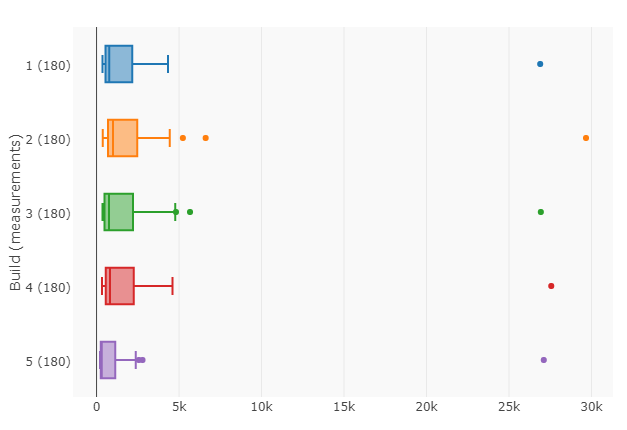
\includegraphics[width=\columnwidth]{travis_builds}
        \caption{Response times in 5 consequent Travis builds in the \zee case study}
        \label{fig:builds}
      \end{figure}

  
  While this integration testing environment is different from the actual production deployment one, and the load used is purely synthetic, as will show in Section~\ref{sec:evaluation}, it can actually be used successfully as an early performance indicator for the application developer. \ins{Although predicting the performance of the application would require advanced statistical work, it can be succesfully used as an advanced warning system for the overall performance trend for given endpoints}.  


  \paragraph{Integration with Travis}
  \ml{added new section... also, this has to be moved after introducing the pre-emptive monitoring since it's about running tests. switched the order}
  

  \ins{The pre-emptive monitoring system} can be configured to work together with Continuous Integration (CI) frameworks like Travis\footnote{\url{https://travis-ci.org/}} that deal with automated integration testing.
  The developer needs to define the unit test folder of the project, the URL that Travis should use for reporting its results, and the number of iterations for each unit test should be executed in order to generate a load for the application. 
  
  Each time a new build is created through Travis, the \tool automatically detects all available unit tests defined by the application developer and iterates through each one of them the number of times predefined by the developer while monitoring the response times for each request. The resulting measurements are persisted in a separate part of the tool database so as not to contaminate the ``live'' monitoring data. Beyond seeing the results of each Travis build in the \tool, this feature also allows for preemptive monitoring of the application, as we discuss in the following.    

  \ins{Besides functioning as an early warning system for performance, tracking the evolving performance of API tests serves a second purpose. To function as an anchor when the developer analyzes performance degradations. For example, when a developer sees that a given endpoint has become less performant after in a newly deployed version, they are able to investigate whether the performance degradation is visible also with the synthetic load. This would correspond to a performance degradation which is due to ``algorithmic performance degradation''. If on the other hand, the performance of the tests does not change between versions, the developer might conclude that the performance degradation could be due to the workload on the machines, or maybe to the workload mix of the users}
  
  %By these means, an application developer can use unit tests as synthetic loads for driving the performance monitoring of the application before it reaches the production phase.  As we will discuss further in Section~\ref{sec:testing}, this feature is integral in enabling preemptive performance monitoring of the application.  
  

  

\section{Performance Perspectives}
\label{sec:views}

  There are three main categories of visual perspectives that are available using \tool:
  \begin{enumerate}
    \item \textit{Service Utilization} presents information about the usage of all endpoints of interest to the developer,
    \item \textit{Endpoint Performance} presents response times of the various service endpoints, and
    \item \textit{User Experience} presents information about the user-perceived performance of monitored service endpoints.
  \end{enumerate}

  %In the remainder of the paper we present several of these perspectives.\footnote{We recommend obtaining a color version of this paper for better readability}

  % The second endpoint conists of two parts, one of them being a table that shows for every monitored endpoint the number of hits it has gotten, the time it was last accessed and its average execution time. The second part is a view with four graphs which show:
  % \begin{itemize} 
  %   \item A heatmap of the total number of requests to the monitored endpoints
  %   \item A stacked bar chart that shows the total number of requests to the monitored endpoints per endpoint per day
  %   \item A boxplot graph showing the average execution time per version of the web service
  %   \item A boxplot graph showing the average execution time for every monitored endpoint
  % \end{itemize}

\todo{Summarize the subsections extensively; evaluate which figures to keep and ideally take new screenshots for the ones we keep; consider adding two more views (like Fig. 3.2 of Patrick's thesis)}

\begin{figure*}[t]
	\centering
	\subfloat[number of requests per endpoint per day]{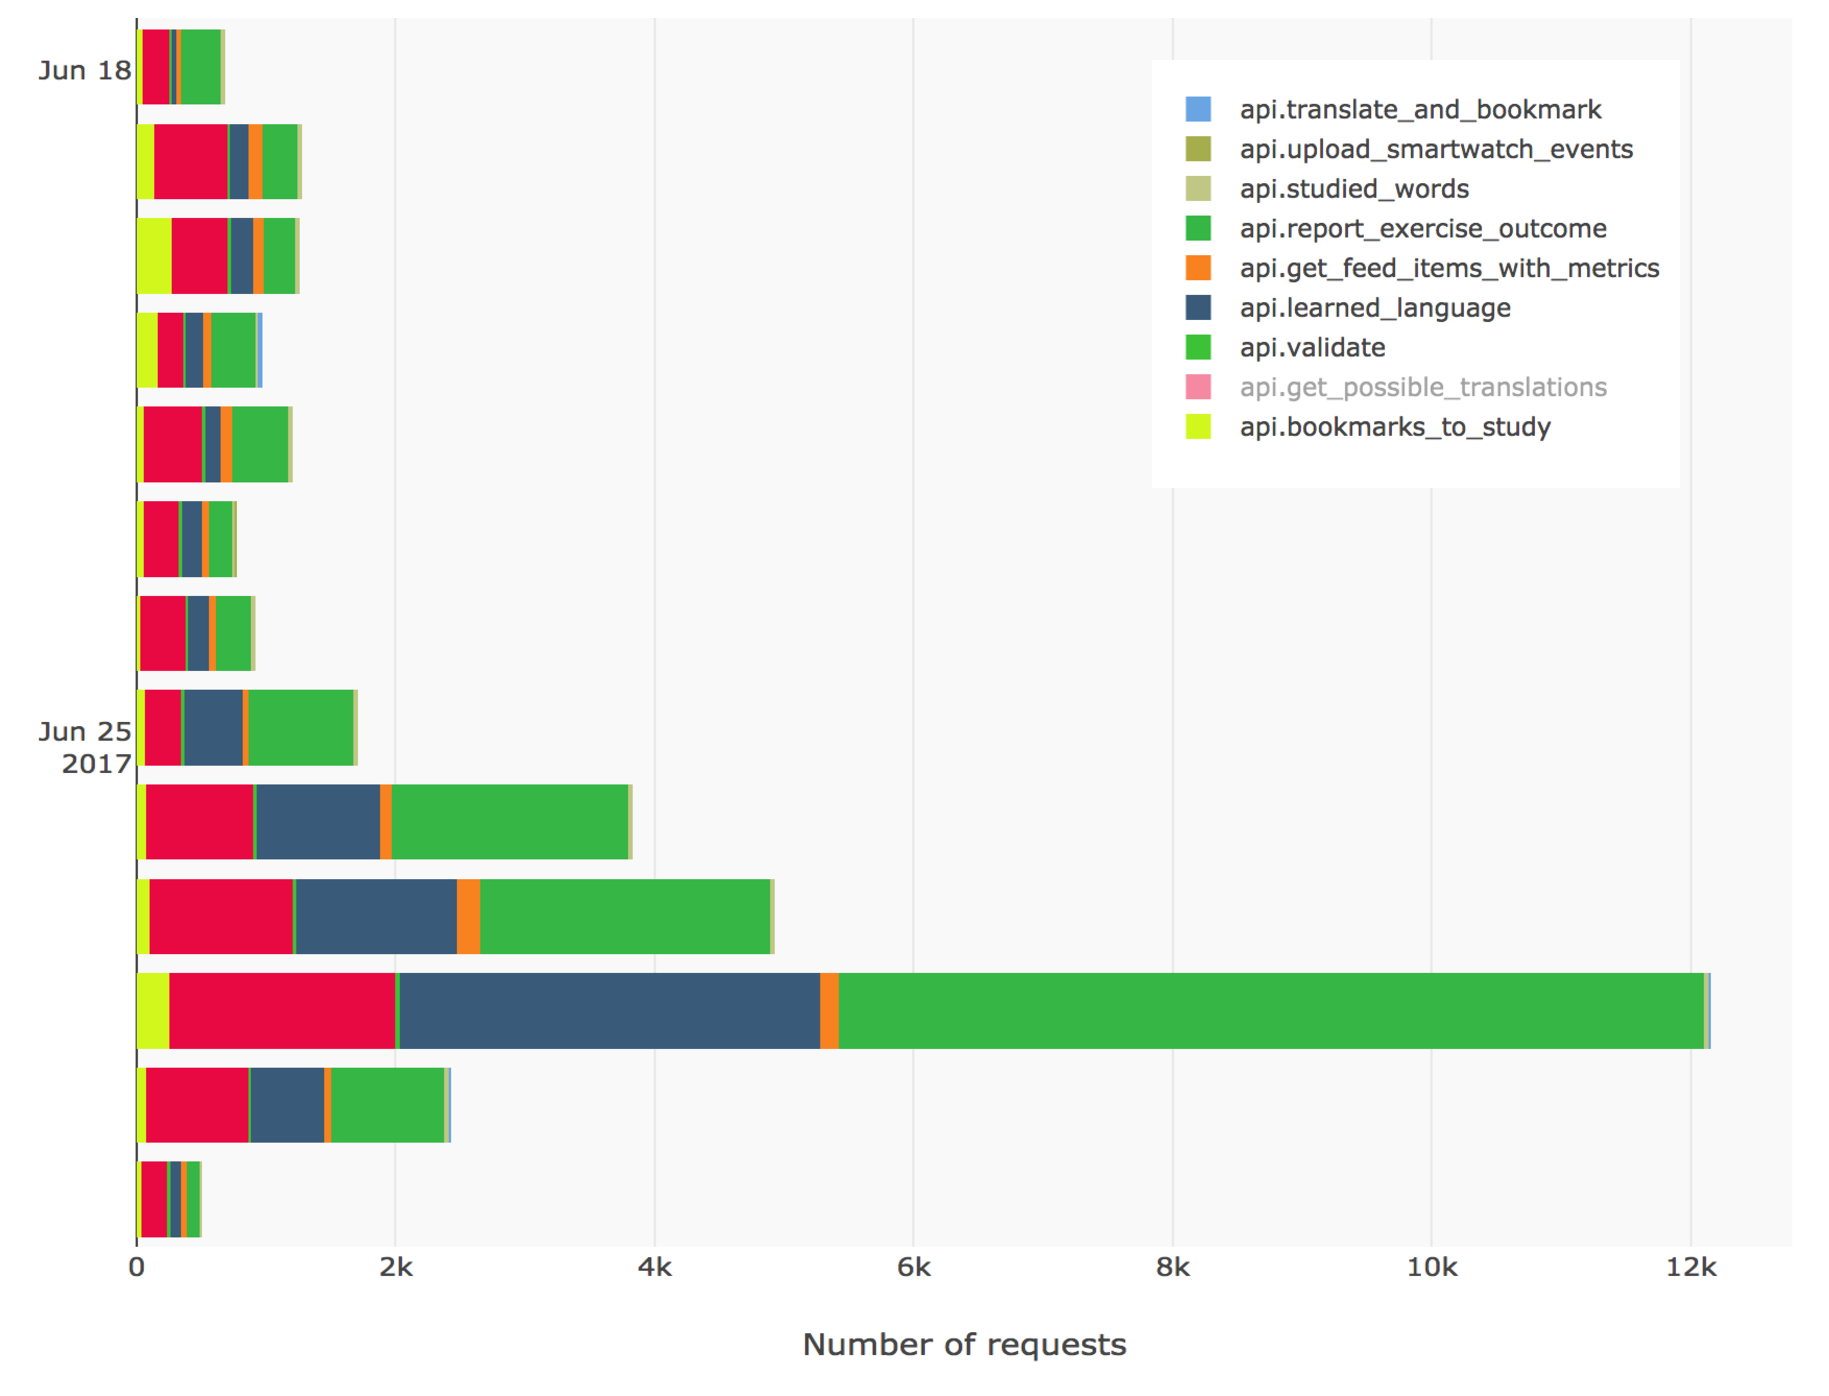
\includegraphics[width=.9\columnwidth]{number_of_requests_}\label{fig:aeu}}
	\subfloat[requests per hour heatmap]{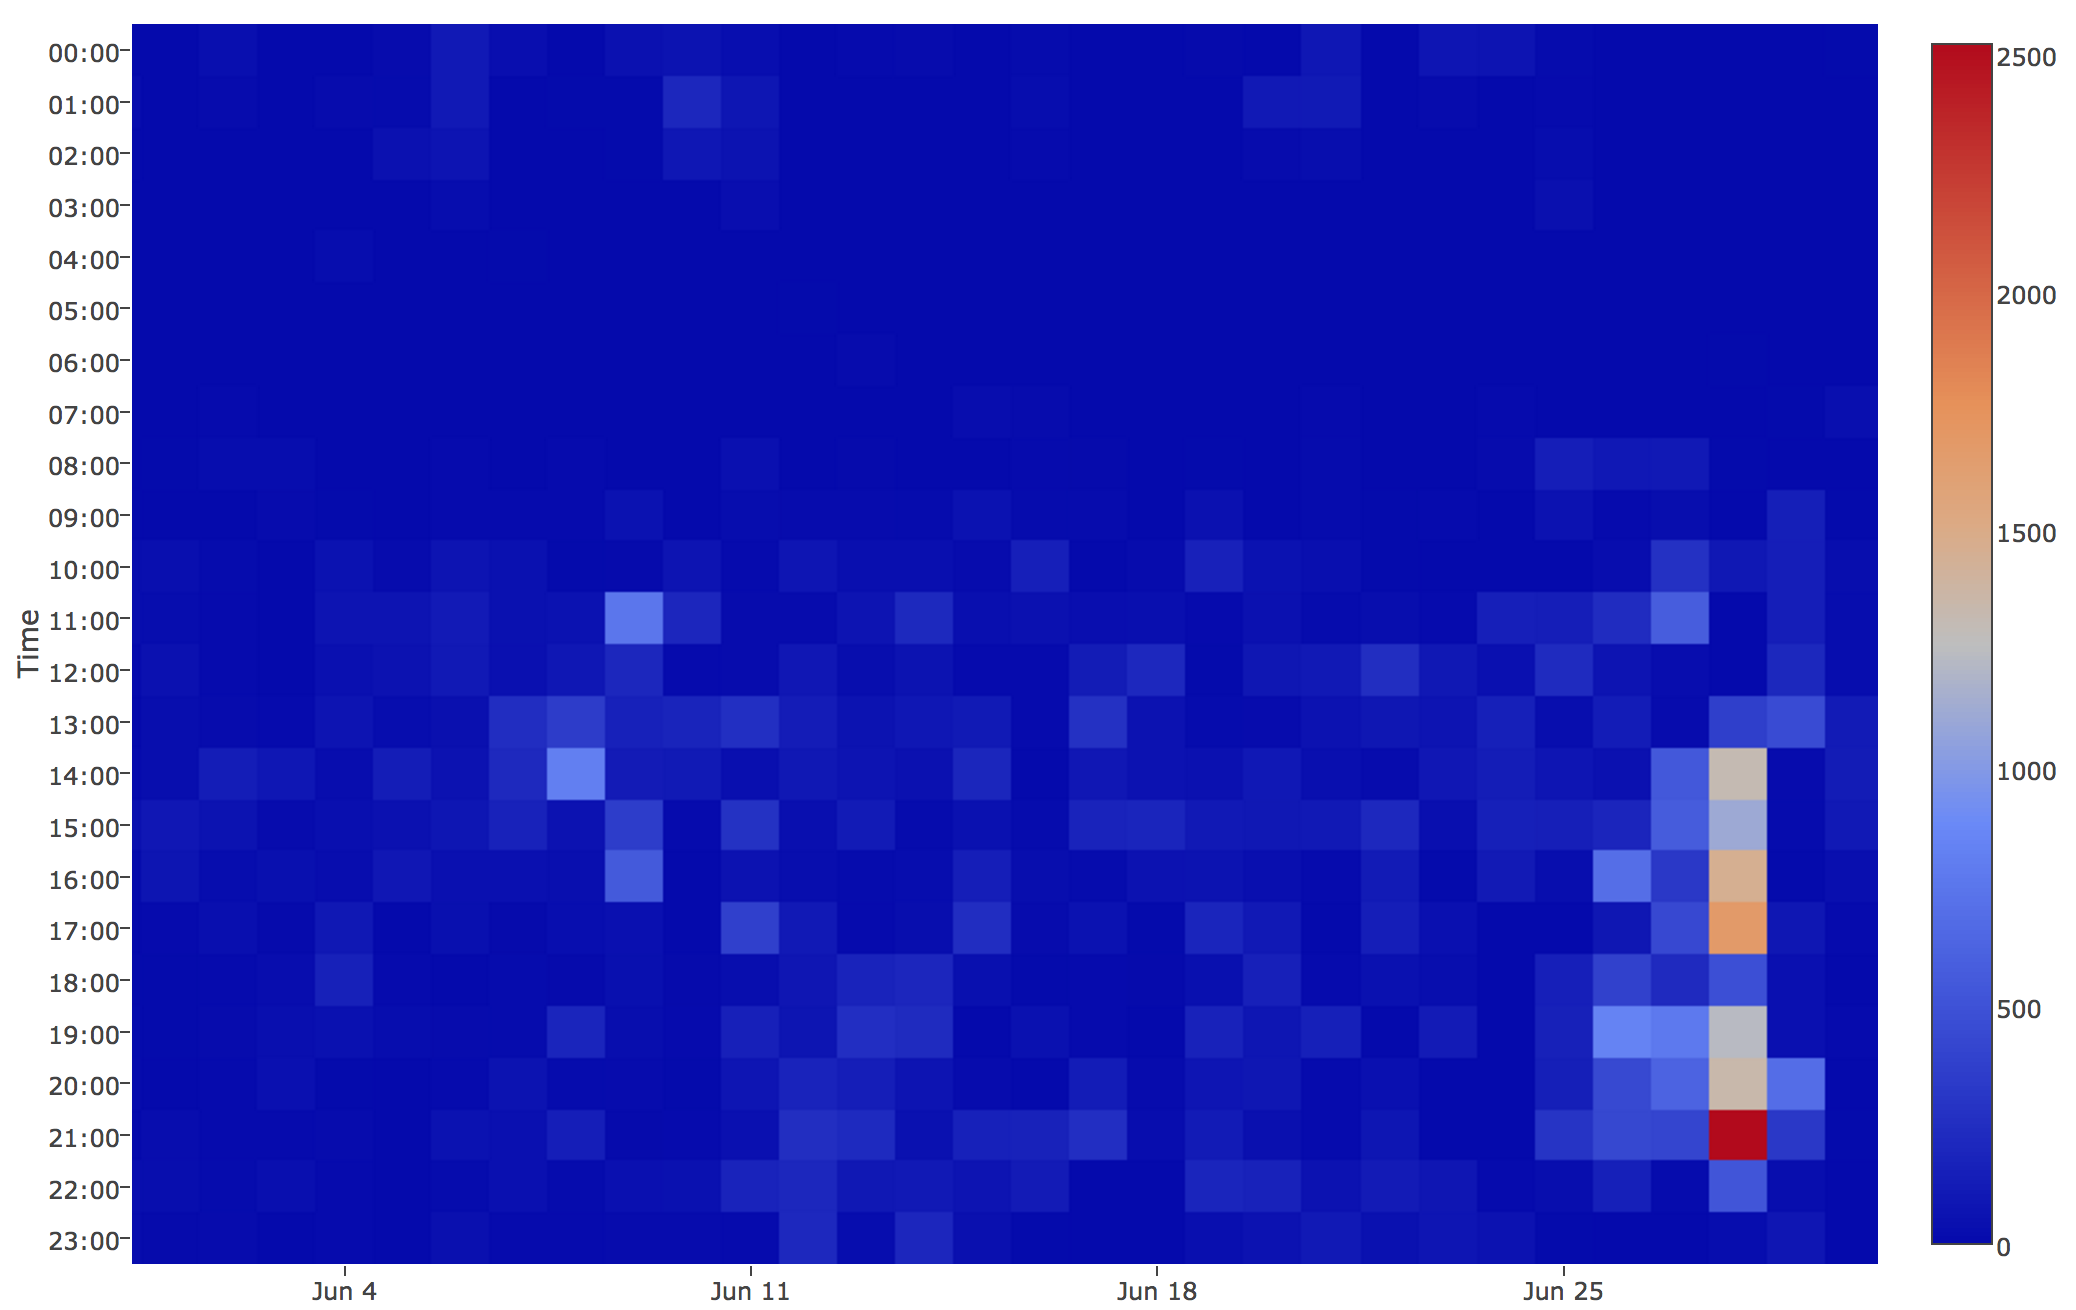
\includegraphics[width=\columnwidth]{daily_patterns_}\label{fig:dp}}
	\qquad
	\subfloat[response time (in ms) per monitored endpoint view]{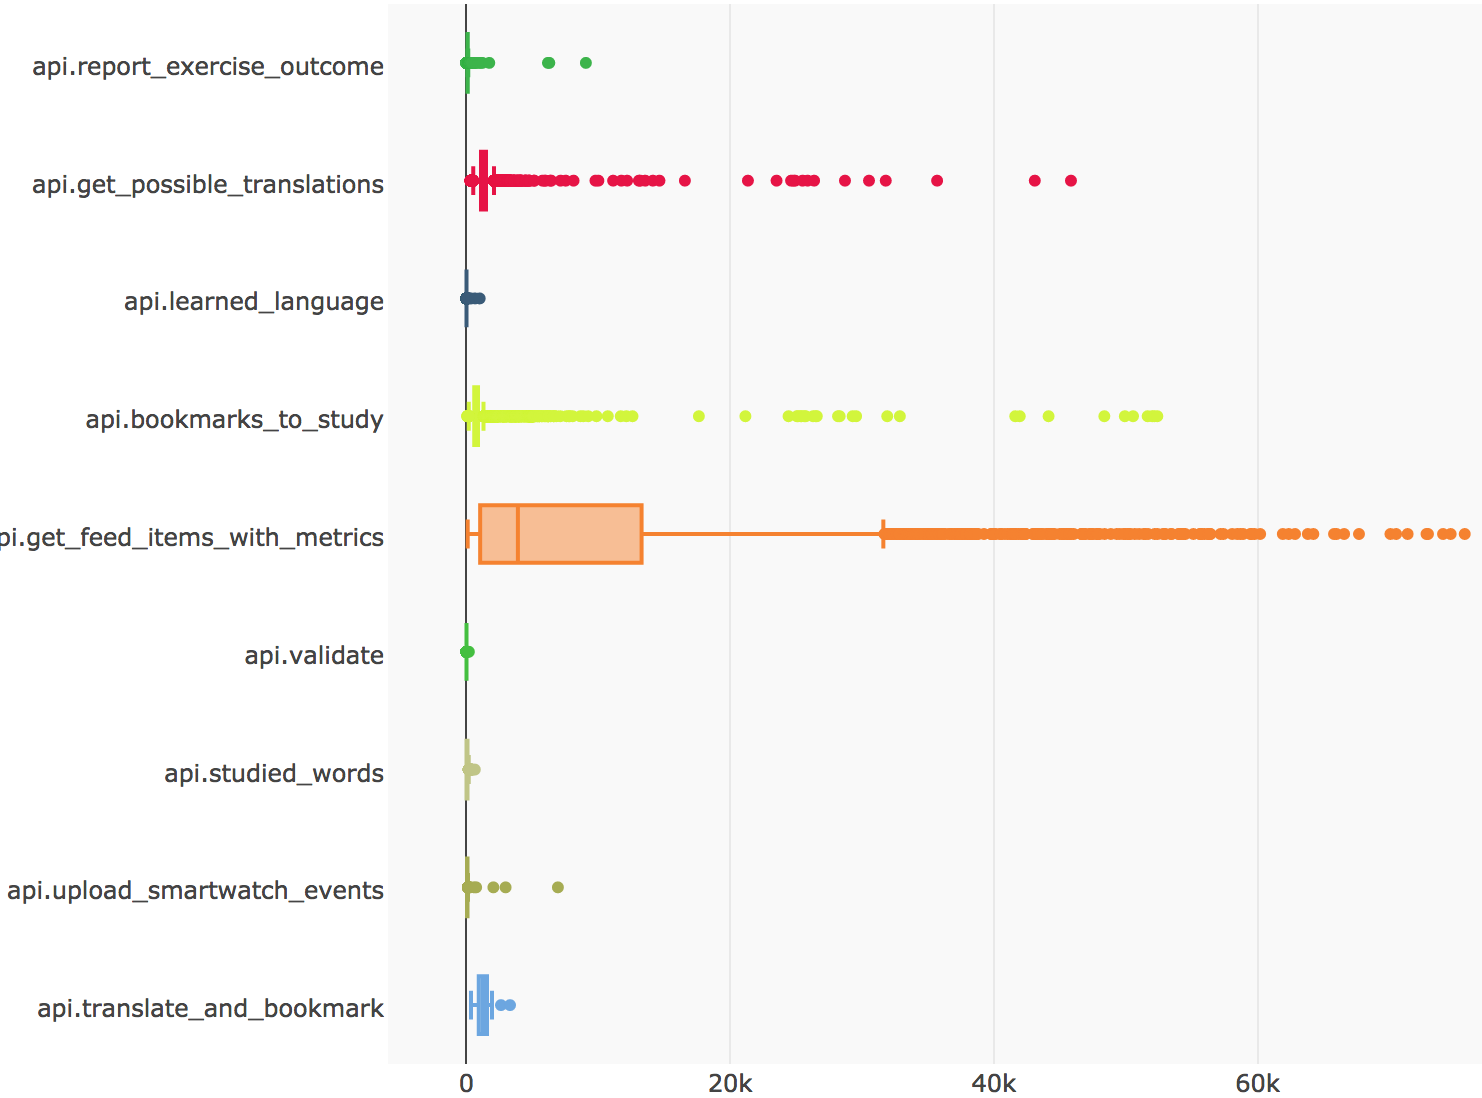
\includegraphics[width=.8\columnwidth]{endpoint_performance_}\label{fig:ep}}\qquad
	\subfloat[The Performance Evolution of the \epTranslations endpoint]{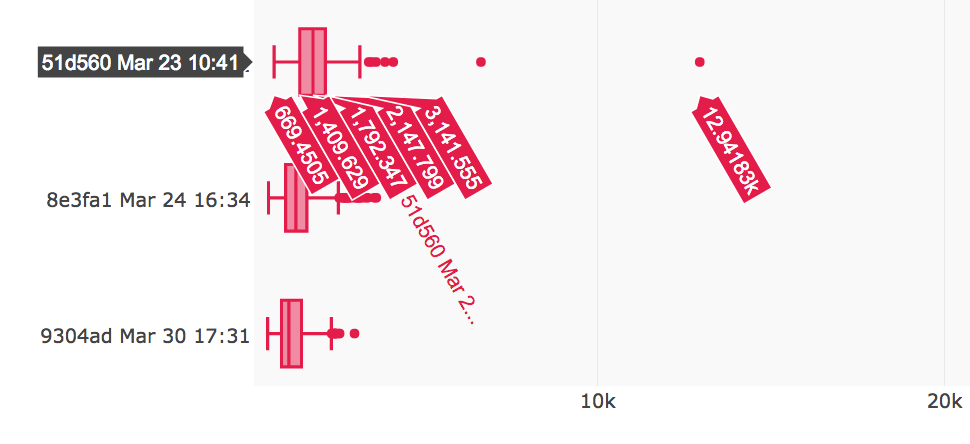
\includegraphics[width=.95\columnwidth]{translation_endpoint_evolution_}\label{fig:tee}}
	\caption{Some of the available views\label{fig:views}}
\end{figure*}

     



\paragraph{Service Utilization}
\label{sec:util}

The most fundamental insight that a service maintainer needs regards service utilization. %\vspace{0.5cm}

Figure \ref{fig:aeu} shows a first perspective on endpoint utilization that \tool provides: a stacked bar chart of the number of hits to various endpoints grouped by day\footnote{Endpoint colors are the same in different views}. Figure~\ref{fig:aeu} in particular shows that at its peak the API has about 12.000 hits per day. 
The way users interact with the platform can also be inferred since the endpoints are indicators of different activity types, e.g.: 

\begin{enumerate}
	
	\item {\color{myred} \epTranslations} is an indicator of the amount of foreign language reading the users are doing, and 
	
	\item {\color{mygreen} \epOutcome} is an indicator of the amount of foreign vocabulary practice the users are doing.
	
\end{enumerate}


%\begin{figure}[!ht]
%	\centering
%	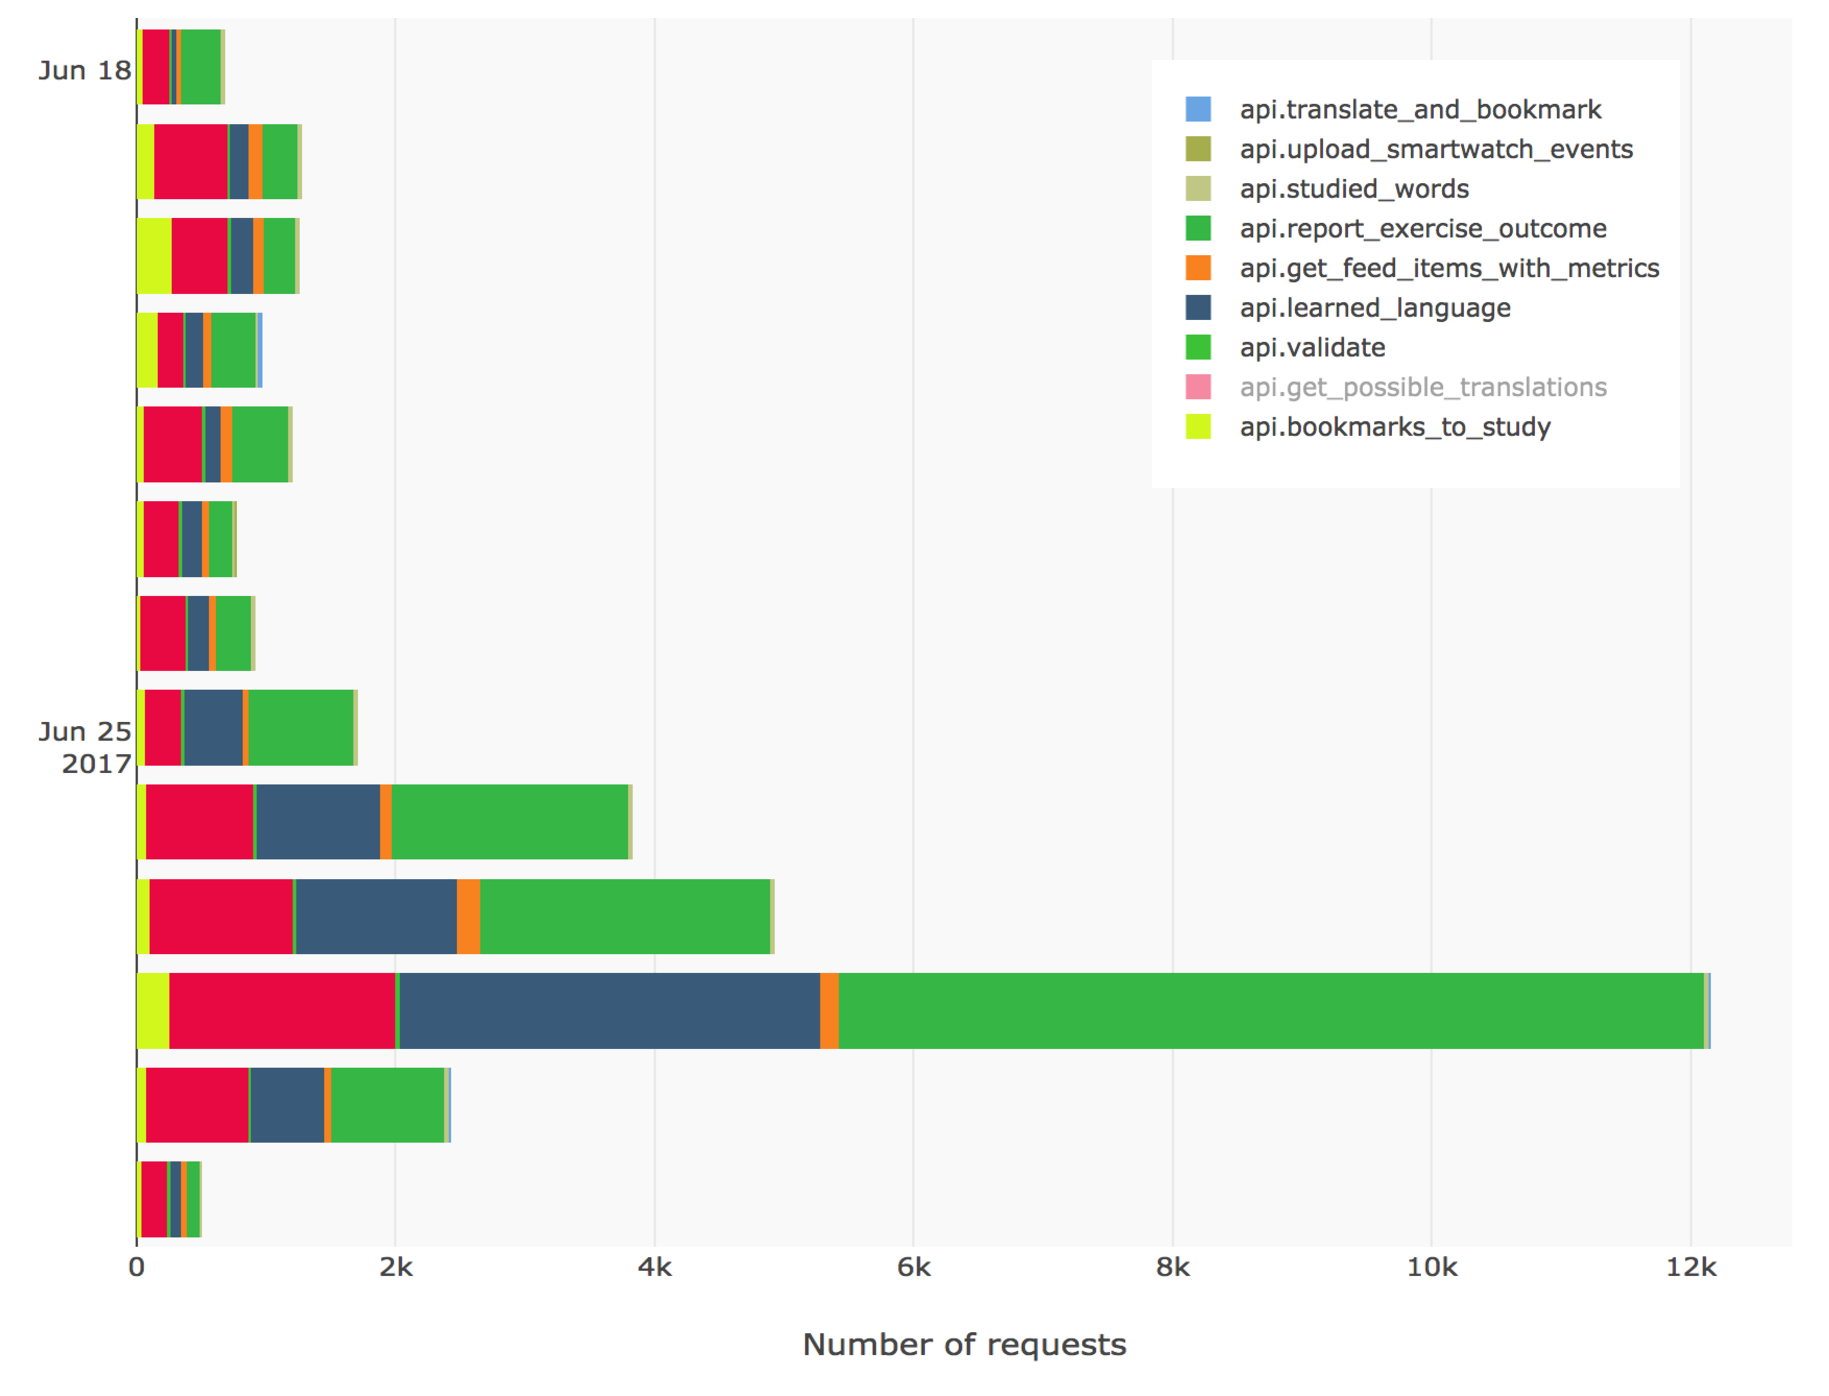
\includegraphics[width=\linewidth]{number_of_requests_}
%	\caption{The number of requests per endpoint per day view shows the overall utilization of the monitored application}
%	\label{fig:aeu}
%\end{figure}

Besides showing the overall utilization, this endpoint provides the maintainer with information relevant for decisions regarding endpoint deprecation --- one of the most elementary ways of {\em understanding the needs of the downstream}\cite{Haen14a}. In our case study, the maintainer realized that one endpoint which they thought was not being used (i.e. \code{words\_to\_study}), contrary to their expectations, was actually being used\footnote{A complementary type of usage information can also be discovered in the view presented in Figure \ref{fig:sep} where seeing that an endpoint is never accessed can increase the confidence of the maintainer that a given endpoint is not used, although it can never be used a proof.}.

\niceseparator

%   \todo{Add the time series graph and discuss it before the heatmap? We can then sell the heatmap better} 
%   \ml{Not sure about which graph you refer to here V}

A second type of utilization question that the \tool can answer automatically regards {\em cyclic patterns of usage per hour of day} by means of a heatmap, as in \Fref{fig:dp}. 

% \mltp{ can we add vertical lines that highlight the beginning of a new week (e.g. before Sunday): }
% Patrick: adding separators in the graph is unfortunately not supported by the library.

%\begin{figure}[!ht]
%	\centering
%	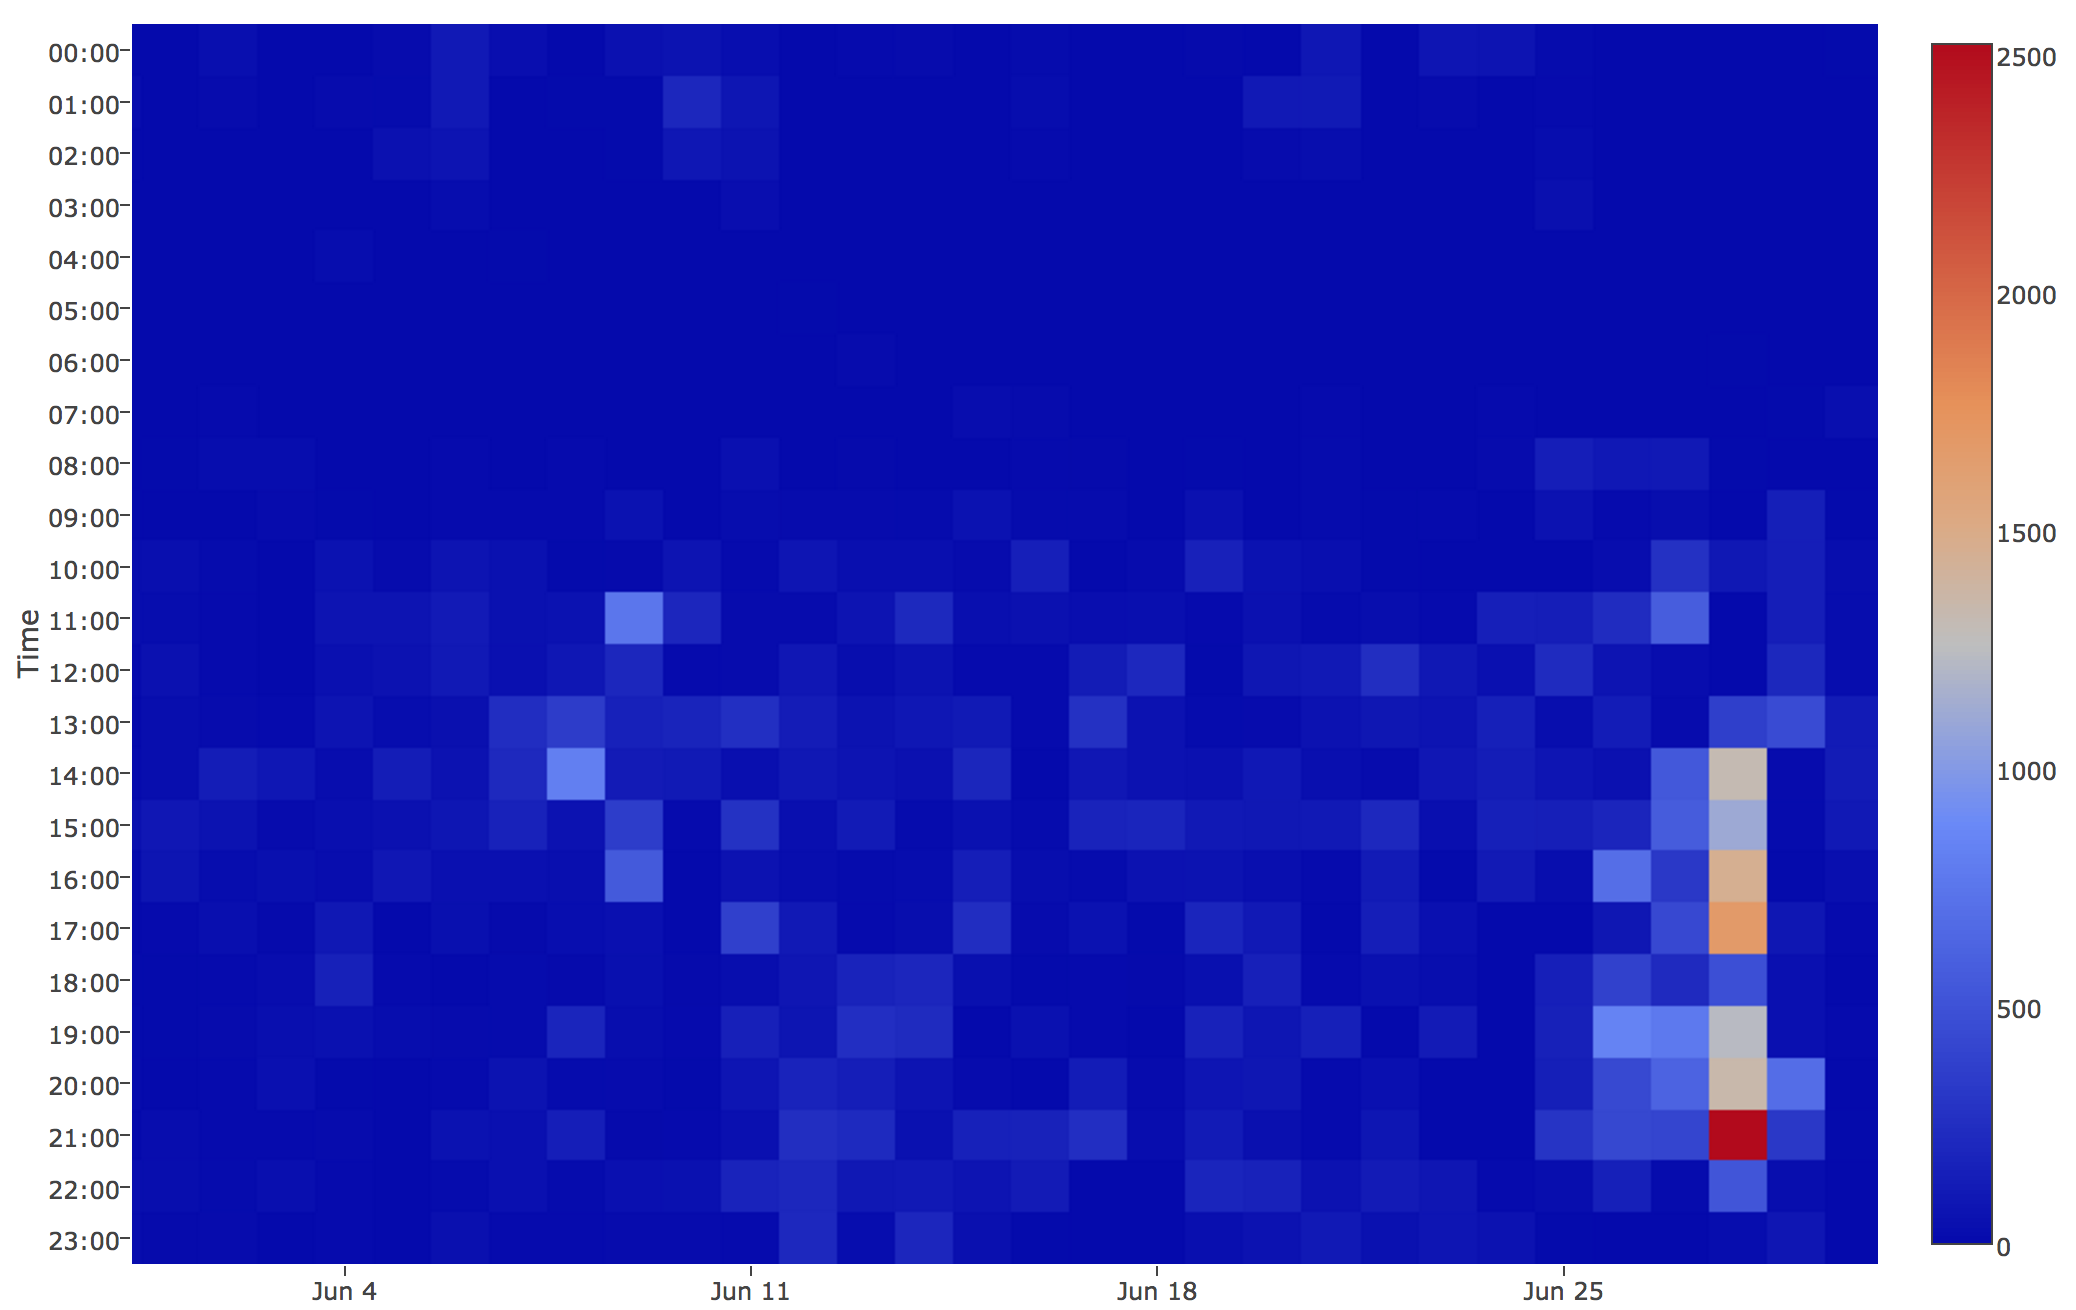
\includegraphics[width=0.9\linewidth]{daily_patterns_}
%	\caption{Usage patterns become easy to spot in the requests per hour heatmap}
%	\label{fig:dp}
%\end{figure}


Figure \ref{fig:dp} shows the API not being used during the early morning hours, with most of the activity focused around working hours and some light activity during the evening. This is consistent with the fact that the current users are all in the central European timezone. Also, the figure shows that the spike in utilization that was visible also in the previous graph happended in on afternoon/evening.

\paragraph{Endpoint Performance}
\label{sec:perf}

  The \tool also collects information regarding endpoint performance. The view in \Fref{fig:ep} summarizes the response times for various endpoints by using a box-and-whiskers plot. 

  % \ml{Thijs and Patrick... the visualization people will complain when they see that we have different colors for the same endpoint in different graphs. Can we insure that there is consistency in colors? Simplest trick would be to obtain the color by hashing the name of the endpoint... in that case the same endpoint would have the same color in various graphs.}
  % This is supported in the latest version of the dashboard

%  \begin{figure}[!ht]
%    \centering
%    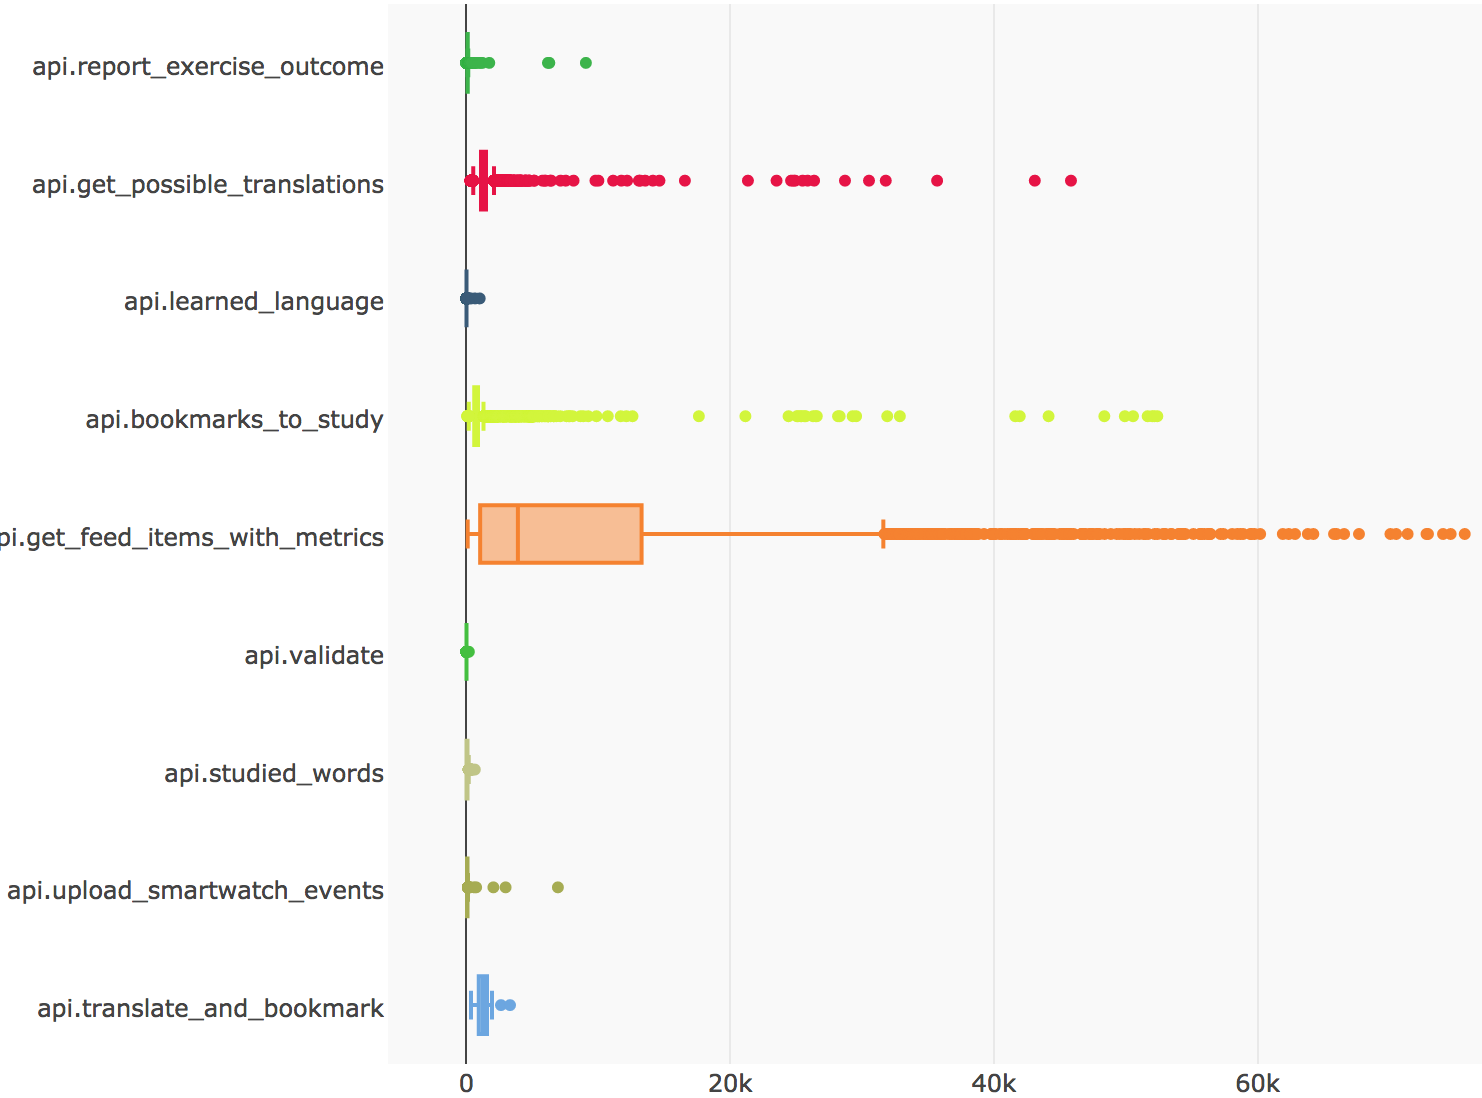
\includegraphics[width=0.95\linewidth]{endpoint_performance_}
%    \caption{The response time (in ms) per monitored endpoint view allows for identifying performance variability and balancing issues}
%    \label{fig:ep}
%  \end{figure}

  From this view it became clear to the maintainer that four of the endpoints had very large variation in performance.   The most critical for the application and consequently the one optimized first was the \epTranslations endpoint which was part of an interactive loop in the reader applications that relied on the Zeeguu API. Moreover, cf. \Fref{fig:aeu} this endpoint is one of the most used in the system.


  \niceseparator

  \todo{remove the part about how to configure git, the discussion has been subsumed by Section~\ref{sec:tool}.}

  However, with the current configuration of the tool, it would be impossible for the maintainer to see the improvements resulting from the optimization. One way to do this is to add an extra line of configuration to allow \tool to find the git\footnote{\url{https://git-scm.com/}} folder of the deployed service: 

%  \begin{lstlisting}[caption=Configuring the \tool with the path to the .git folder enables the generation of evolutionary performance graphs, style=custompython]
%
%dashboard.config.git = 'path/to/.git'
%
%
%    \end{lstlisting}
    
    \begin{lstlisting}[style=custompython]
  
  dashboard.config.git = 'path/to/.git'
    
  \end{lstlisting}  
 
  With this extra configuration, the \tool can now automatically detect the current version of the project, and group measurements by version\footnote{Alternatively, the maintainer can add version identifiers manually for the web application through a configuration file if the system does not use git.}. \Fref{fig:tee} is a zoomed-in version of such a view for \epTranslations with versions increasing from top to bottom
  
  
%    \begin{figure}[h!]
%      \centering
%      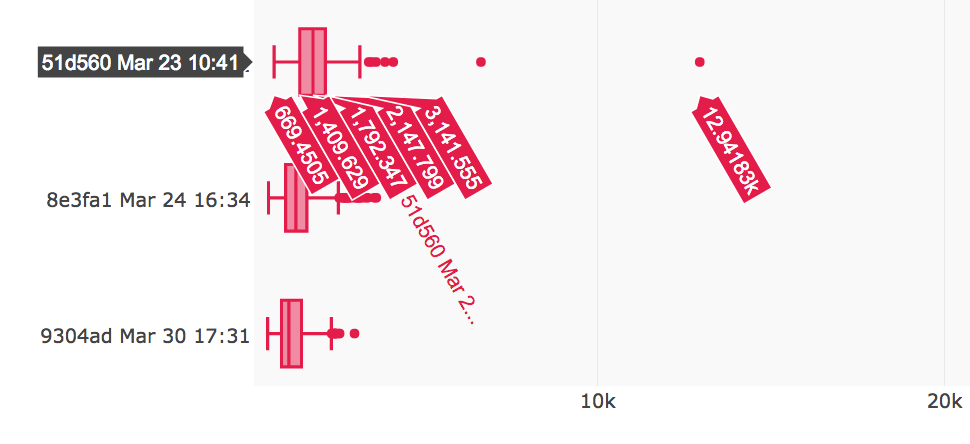
\includegraphics[width=0.95\linewidth]{translation_endpoint_evolution_}
%      \caption{Visualizing The Performance Evolution of the \epTranslations endpoint}
%      \label{fig:tee}
%    \end{figure}

  This view confirms that the performance of the translation endpoint improved in the recent versions: the median of the last three versions is constantly moving towards the left, and progresses from 1.4 seconds (in the top-most box plot in \Fref{fig:tee}) to 0.8 in the latest version (bottom-most box plot).
  

\paragraph{User Experience}
\label{sec:user}

For service endpoints which run computations in real time, the maintainer of a system might want to understand the endpoint performance on a per-user basis, especially for situations where the system response time is a function of some individual user load\footnote{E.g. in GMail some users have two emails while other have twenty thousand and this induces different response times for different users}.

\todo{remove the configuration part and rephrase the following, the discussion has been partially subsumed by Section~\ref{sec:tool}.}

To enable this, the \tool must be configured to associate an API call with a given user. The simplest way is to take advantage of the architecture of Flask applications in which a global \code{flask.request} object can be used to retrieve the session which can in turn lead to user identification: 

%\begin{lstlisting}[float,caption=Simply define a custom app-specific function for user retrieval and pass it to the \tool to group information by user,style=custompython]
\begin{lstlisting}[style=custompython]  
# app specific way of extracting the user
# from a flask request object    
def get_user_id():
sid = int(flask.request.args['session'])
session = User.find_for_session(sid)
return user_id

# attaching the get_user_id function
dashboard.config.get_group_by = get_user_id

\end{lstlisting}

% \niceseparator

\todo{consider losing one or both of the figures --- or at least updating them}

In Zeeguu, \epFeedItems retrieves a list of recommended articles for a given user. Cf. \Fref{fig:ep} it is the endpoint with the slowest response time and highest variability. The reason for this is that a user can be subscribed to anything from one to three dozen article sources and for each of the sources the system must compute the personalized difficulty of each article at every request. 

% In the Zeeguu case study, one of the slowest endpoints, and one with the highest variability as shown in \Fref{fig:ep} is \epFeedItems: it retrieves a list of recommended articles for a given user. However, since a user can be subscribed to anything from one to three dozen article sources, and since the computation of the difficulty is personalized and it is slow, the variability in time among users is likely to be very large. 


\begin{figure}[!ht]
	\centering
	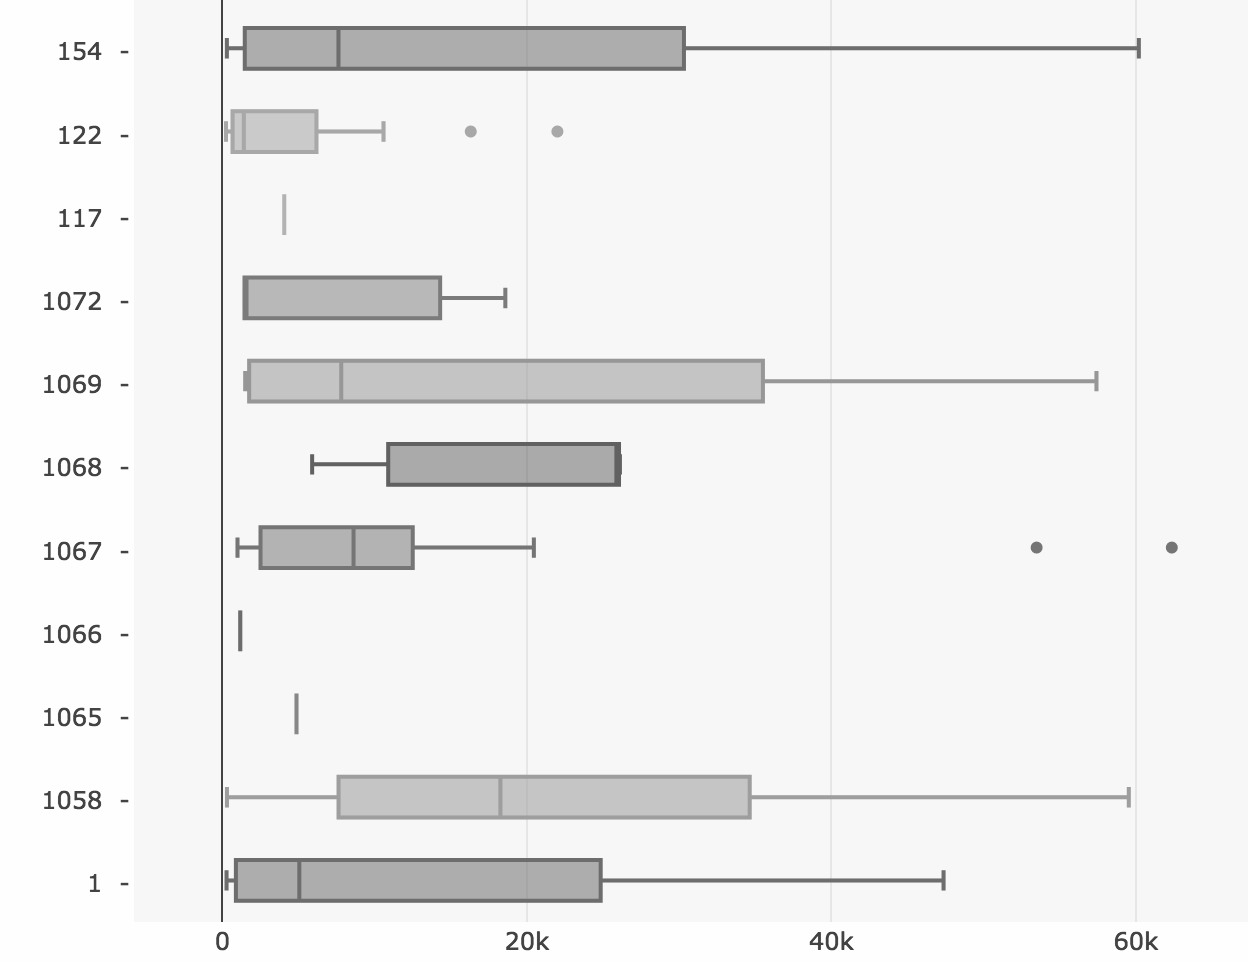
\includegraphics[width=0.85\linewidth]{time_per_user}
	\caption{The \epFeedItems shows a very high variability across users}
	\label{fig:tpu}
\end{figure}

A \perspective{Per-User Performance} perspective should show the different response times for different users. Figure \ref{fig:tpu} presents a subset of the corresponding view in the \tool. The figure shows that the response times for this endpoint can vary considerably for different users with some extreme cases where a user has to wait a full minute until their recommended articles are shown\footnote{After seeing this perspective, the maintainer refactored the architecture of the system to move part the difficulty computation out of the interactive loop}.


% \niceseparator

The limitation of the previous view is that it does not present the information also on a per version basis. To address this, a different visual perspective entitled \perspective{Multi-Version per-User Performance} can be defined. Figure \ref{fig:tuv} presents such a perspective by mapping the average execution time for a given user (lines) and given version (columns) on the area of the corresponding circle. The colors represent users. The figure shows average performance varying  across users and versions with no clear trend: this is probably because varying user workload (i.e. number of sources to which the user is registered) is the reason for the variation in response times.

\begin{figure}[!ht]
	\centering
	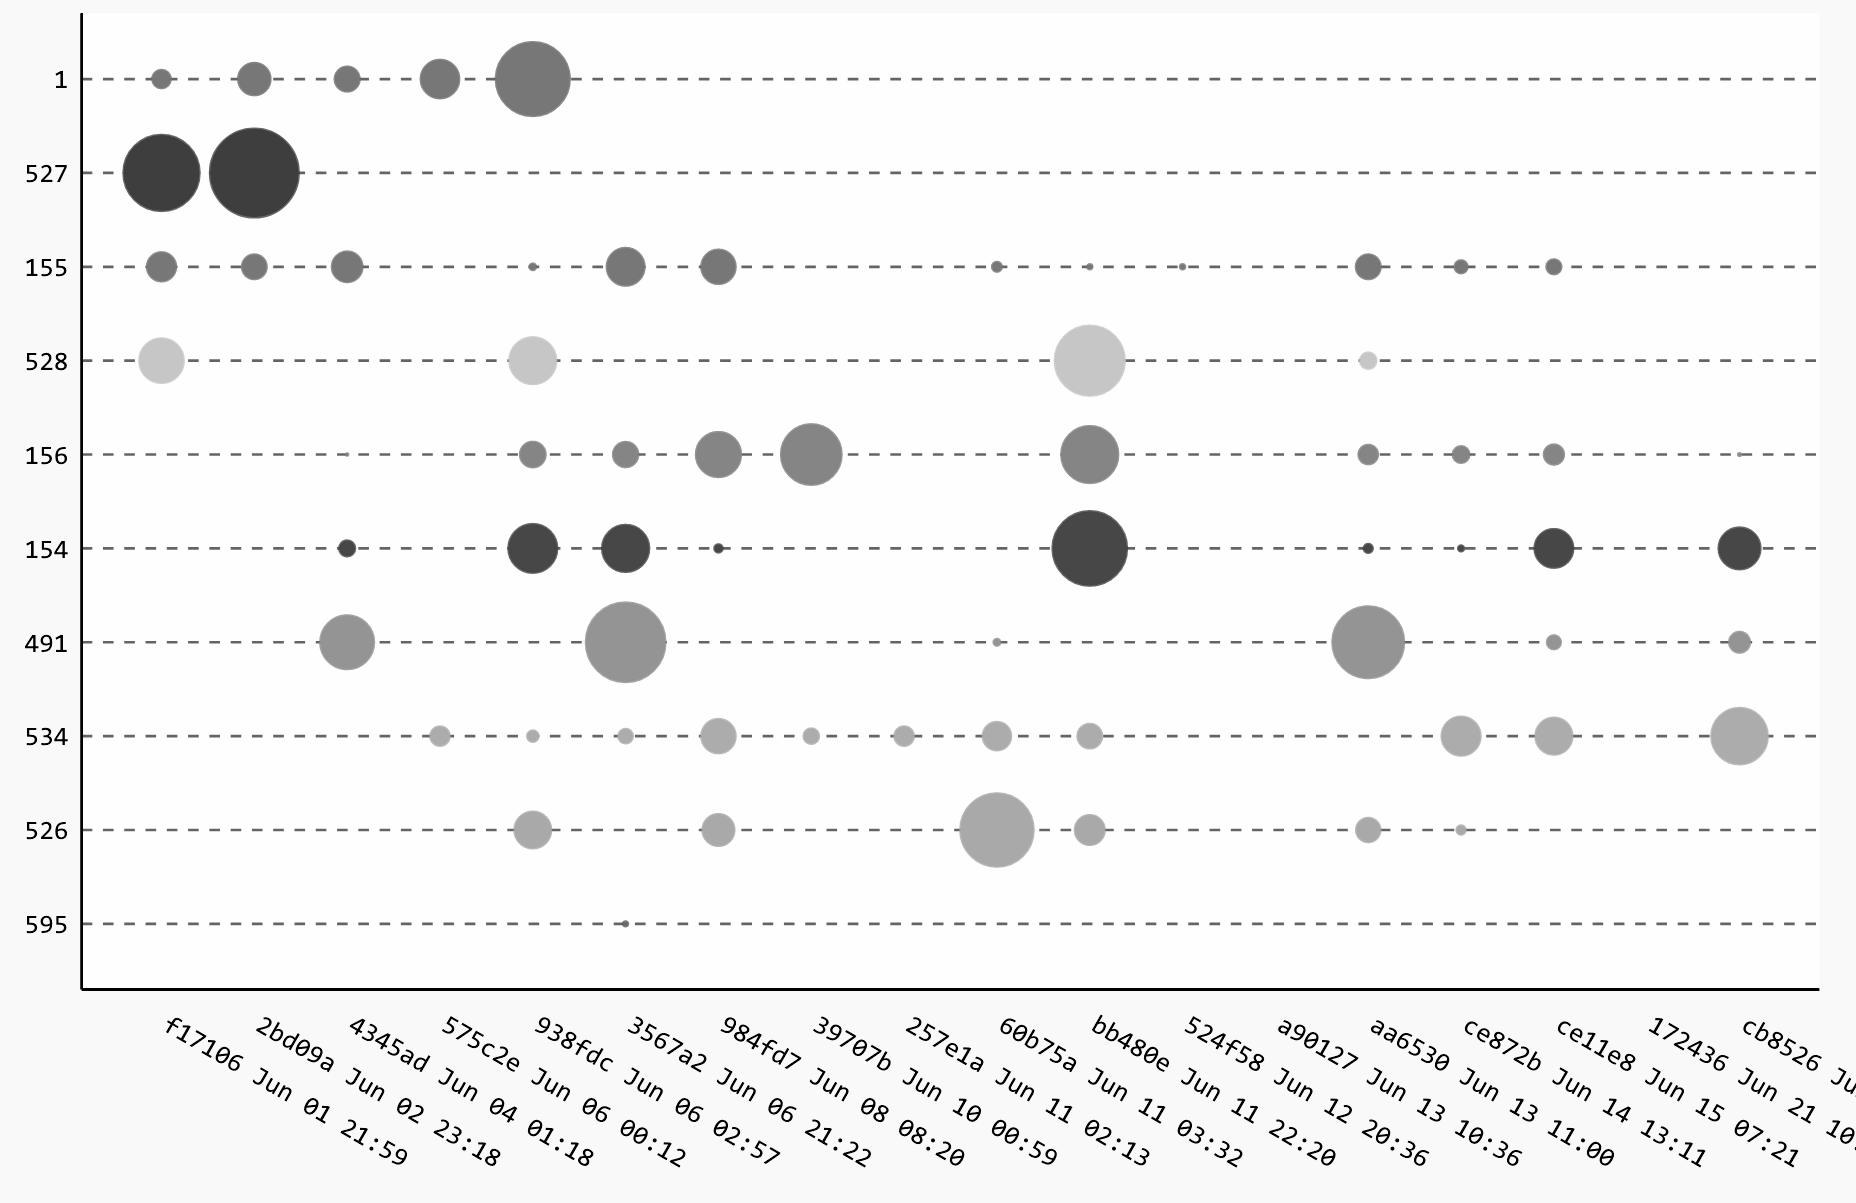
\includegraphics[width=0.9\linewidth]{time_per_user_per_version}
	\caption{This perspective shows that the evolution of response times for individual users (horizontal lines) across versions (the x-axis)}
	\label{fig:tuv}
\end{figure}

%\section{Preemptive Monitoring}
%\label{sec:testing}
%
%%\todo{discuss here idea of using unit testing as an early performance indicator for evolving services (`preemptive monitoring'?); add a side-by-side figure comparing unit testing vs live system performance per version, maybe calculate error in trend curves? find a better term than prediction for the section title (plus introduction)}
%
%\todo{Similar to the idea of augmenting service monitoring with online testing~\cite{metzger2010proactive}, i.e.~testing service-based applications by using dedicated test input in parallel to its normal use and operation. The difference is that we take advantage of the capability of Travis to create an emulated live environment for integration testing purposes, and use unit testing as the dedicated test input in order to measure performance. What we are going provide evidence for in the following is that we can indeed use this preemptive monitoring concept as an early performance indicator for evolving services.}
%
%The developer needs to define the unit test folder of the project, the URL that Travis should use for reporting its results, and the number of iterations for each unit test should be executed in order to generate 


\section{Evaluation}
\label{sec:evaluation}

%\todo{evaluation of the \tool across the following dimensions: ease of use, effectiveness, overhead to the system; for the last part we need to do the overhead measurement experiment, for the other two we base it on the case study and bring over whatever is necessary from the discussion section}

\subsection{Effectiveness \& Ease of Use}

\todo{@M: move here the war stories, and discuss how useful the whole thing was to the application maintainer}

\subsection{Efficiency of Preemptive Monitoring}

\todo{here goes the discussion about our forecasting capabilities}

\begin{figure}
	\centering
	\subfloat[The reported response time (in ms) per deployed version in the observation period]{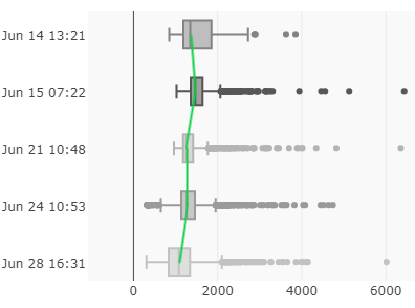
\includegraphics[width=.5\columnwidth]{response_per_version_trunced_trend}}
	\quad
	\subfloat[The measured response time (in ms) using integration with Travis]{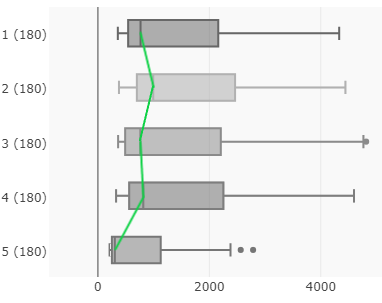
\includegraphics[width=.46\columnwidth]{travis_builds_no_outliers_trend}}
	\caption{Comparison of the response times per endpoint: actual production system versus preemptive monitoring data}
	\label{fig:preemptive}
\end{figure}


\begin{table}[h]
	\begin{tabular}{lll}
		\toprule
		Iteration & \bfseries Live (median) & \bfseries Travis (median)\\
		\midrule
		1 & 1349.41 & 764.87\\ 
		2 & 1466.13 & 992.87\\
		3 & 1256.65 & 760.87\\
		4 & 1266.42 & 813.89\\
		5 & 1080.68 & 303.4\\
		\bottomrule
	\end{tabular}
\end{table}

Pearson correlation $r(3)=.93, p=.02$

\subsection{Discussion}

\todo{use this subsection to discuss limitations (from the previous evaluation section) and add the need to be able to handle the horizontal scaling of the application; remove sectioning and summarize briefly limitations that have already been discussed in the VISSOFT paper/move material to other sections; consider renaming as limitations or something similar}

  \subsubsection{Automatically Monitoring System Evolution}

  The main goal of the \tool design was to allow analytics to be collected and insight to be gained by making the smallest possible changes to a running API. %To allow the collection of evolutionary information 
%
  This technique assumes that the web application code which is the target of the monitoring is deployed using \git in the following way: 

  \begin{enumerate}
    \item The deployment engineer pulls the latest version of the code from the integration server; this will result in a new commit being pointed at by the HEAD pointer. %than previously
    \item The deployment engineer restarts the new version of the service. At this point, the \tool detects that a new HEAD is present in the local code base and consequently starts associating all the new data points with this new commit\footnote{The \tool detects the current version of the analyzed system the first time it is attached to the application object, and thus, assumes that the Flask application is restarted when a new version is deployed. This is in tune with the current version of Flask, but if the web server will support dynamic updates in the future, this might have to be taken into account}.
  \end{enumerate}

  The advantage of this approach is the need for minimal configuration effort, as discussed in the presentation of the tool. The disadvantage is that it will consider on equal ground the smallest of commits, even one that modifies a comment, and the shortest lived of commits, e.g.~a commit which was active only for a half an hour before a new version with a bug fix was deployed, with major and minor releases of the software. %as a distinct way of grouping the data points. 
  A mechanism to control which versions are important for monitoring purposes is therefore required to be added.
%
  A further possible extension point here is supporting other version control systems (e.g. Mercurial). However, this is a straightforward extension.



  \subsubsection{User-Awareness }

    For the situations in which the user information is not available, the \tool tracks by default information about different IPs and in some cases this might be a sufficiently good approximation of the user diversity and identity. 
    %

    The visualizations for the user experiene perspectives as presented in Section \ref{sec:user} have been tested with several hundred users (of which about \activeUserCount were active during the course of the study), but the scalability of the visualizations must be further investigated for web services with tens of thousands of users.


  \subsubsection{Other Possible Groupings}

    There are other groupings of service utilization and performance that could be important to the maintainer, that we did not explore in this paper. For example, if the service is using OAuth, then together with every request, in the header of the request there is information about the application which is sending a request. Grouping the information by application that sends the request could be important in such a context. 

    In general, providing a mechanism that would allow very easy specification of groupings (either as code annotations, as normal code, or as configuration options) is an open problem that \tool and any other similar library will have to face.



\section{Related Work}
\label{sec:related}

\todo{Refer the reader to~\cite{ghezzi2007run} and ~\cite{metzger2010analytical} for a more extensive discussion}

There is a long tradition of using visualization for gaining insight into software performance. Tools like Jinsight \cite{Pauw02a} and Web Services Navigator \cite{Pauw05} pioneered such an approach for Java and for Web Services that communicate with SOAP messages. Both have an ``omniscient'' view of the services / objects and their interactions. As opposed to them, in our work we present an analytics platform which focuses on monitoring a single Python web service from its own point of view.

From the perspective of service monitoring, our work falls within the server-side run-time monitoring of services ~\cite{ghezzi2007run}. While we don't implement the more advanced features of related monitoring solutions like QoS policies driving the monitoring, it presents nevertheless an easy to use approach support improving the performance of web applications. 

% \va{Mircea: Consider removing the rest for space...}
% An existing monitoring tool is Pingdom \footnote{https://www.pingdom.com/company/why-pingdom}, which monitors the uptime of an existing web-service. This tool works by pinging the websites (up to 60 times) every minute automatically. Thus this creates a lot of overhead and is bound to be noisy since it will also be influenced by the speed of the network connection\footnote{Another problem is that such a tool would }

% \todo{Runscope? Others?}


\section{Conclusion and Future Work}
\label{sec:conclusions}

\todo{update as appropriate}

In this paper we have shown that it is possible to create a monitoring solution which provides basic insight into web service utilization and performance  with very little effort from the developer. The user group that we are aiming for with this work is application developers using Flask and Python to build web applications with limited or no budget for implementing their own monitoring solutions. The emphasis is in allowing such users to gain insight into how the performance of the service evolves together with the application itself. We believe that the same architecture, and lessons can be applied to other frameworks and other languages.

In the future, we plan to perform case studies with other sytstems, with the goal of discover other needs and to wean out the less useful visualizations in the \tool. We plan to also extend the tool towards supporting multiple deployments of the same applications across multiple nodes (e.g. for the situations where the application is deployed together with a load balancer). Finally, we plan to integrate \tool with unit testing as a complementary source of information about performance evolution.


% references section

\bibliographystyle{abbrv}
\bibliography{soap}


% that's all folks
\end{document}


